%=== CHAPTER TWO (2) ===
%=== Literature Review ===

\chapter{Literature Review}

\section{Visual SLAM}

\subsection{Introduction}
Simultaneous Localizaiton and Mapping (SLAM) is a technique to obtain 3D structure of an unknown environment and sensor motion in the environment. After years of development, SLAM-based application have become widely broadened such as computer vision based 3D modeling, augmented reality(AR)-based visualization and self-driving cars. 

In early SLAM algorithms, there exit many different modalities of sensors integrated in SLAM systems, such as rotary encoders, light detection and ranging radar (LiDAR), inertial sensors, GPS and cameras. In recent years, SLAM using cameras only,  specifically referred to as visual SLAM (vSLAM), has been actively discussed because the sensor configuration is simple, low-cost, and contains abundant information. But meanwhile this technique also brings more difficulties than others using integrated sensors\cite{taketomi2017visual}. 

vSLAM algorithms have proposed widely in the field of computer vision, robotics and AR. The low requirement on the modalities of sensors, requiring cameras only, is the major advantage of vSLAM technique, so that it is very suitable for low-cost unmanned vehicles, robots with limited load capacity and power supply like drones, or mobile devices such as camera-mounted tablets or smart phones.

However, the difficulties brought by vSLAM can not be ignored. Instead of obtaining depth and location information directly from LiDAR, GPS or depth camera in integrated SLAM systems, vSLAM technique needs to compute all these information from color or gray images, which reduces stability and accuracy for several estimation steps involved in this process. Also obviously the computational cost are significantly higher. Therefore, the problem of how to improve the performance and reduce computational cost of vSLAM has always been widely concerned.

\subsection{Feature-based Algorithm}

\subsection{Segmentation-based Algorithm}

\subsection{ORB-SLAM}
\label{chp:orbslam}
One of the state-of-the-art vSLAM solutions for single-robot systems is ORB-SLAM, initially proposed in \cite{mur2015orb}, and upgraded to a second version in \cite{mur2017orb}.

ORB-SLAM is a feature-based monocular SLAM system that operates in real time, in small and large, indoor and outdoor environments. Upgraded to ORB-SLAM2 in \cite{mur2017orb}, the new vision is capable of processing monocular, stereo and RGB-D input. In the proposed work in \cite{mur2015orb}, ORB-SLAM is built on the main ideas of PTAM, the place recognition work of G\'alvez-L\'opez and Tard\'os \cite{galvez2012bags}, the scale-aware loop closing of Strasdat et. al \cite{strasdat2010scale} and the use of covisibility information for large scale operation \cite{strasdat2011double}, \cite{mei2010closing}. As a novel monocular SLAM system, the main contributions of ORB-SLAM are:
\begin{enumerate}[1.]
	\item The same features are used in all tasks: tracking, mapping, relocalization and loop closing. Using same features makes the system more efficient, reliable and simple. And using ORB features allows real-time performance without GPUs, with good invariance to changes in viewpoint and illumination.
	\item Real time performance in large environments. The tracking and mapping modules focus in a local covisible area, independent of the global map, thanks to the use of a covisibility graph.
	\item Real time loop closing. The optimization of a pose graph called the Essential Graph is adapted to realize real time loop closing performance. The Essential Graph is built from loop closures links, strong edges from the covisibility graph and a spanning tree maintained by the system.
	\item Real time camera relocalization with significant invariance to viewpoint and illumination. This allows recovery from tracking failure and also enhances map reuse.
	\item A new automatic and robust initialization procedure based on model selection that permits to create an initial map of planar and non-planar scenes.
	\item A survival of the fittest approach to map point and keyframe selection that is generous in the spawning but very restrictive in the culling. This policy improves tracking robustness, and enhances life-long operation because redundant keyframes are discarded.
\end{enumerate}

ORB-SLAM system, see on Figure \ref{fig:orbslamoverview}, incorporates three threads that run in parallel: tracking, local mapping and loop closing. 

The tracking thread is in charge of localizing the camera with every frame and deciding when to insert a new keyframe.	The module firstly match current frames with previous frames, and optimize the pose using motion-only bundle adjustment. If the 

\begin{figure}[H]
	\centering
	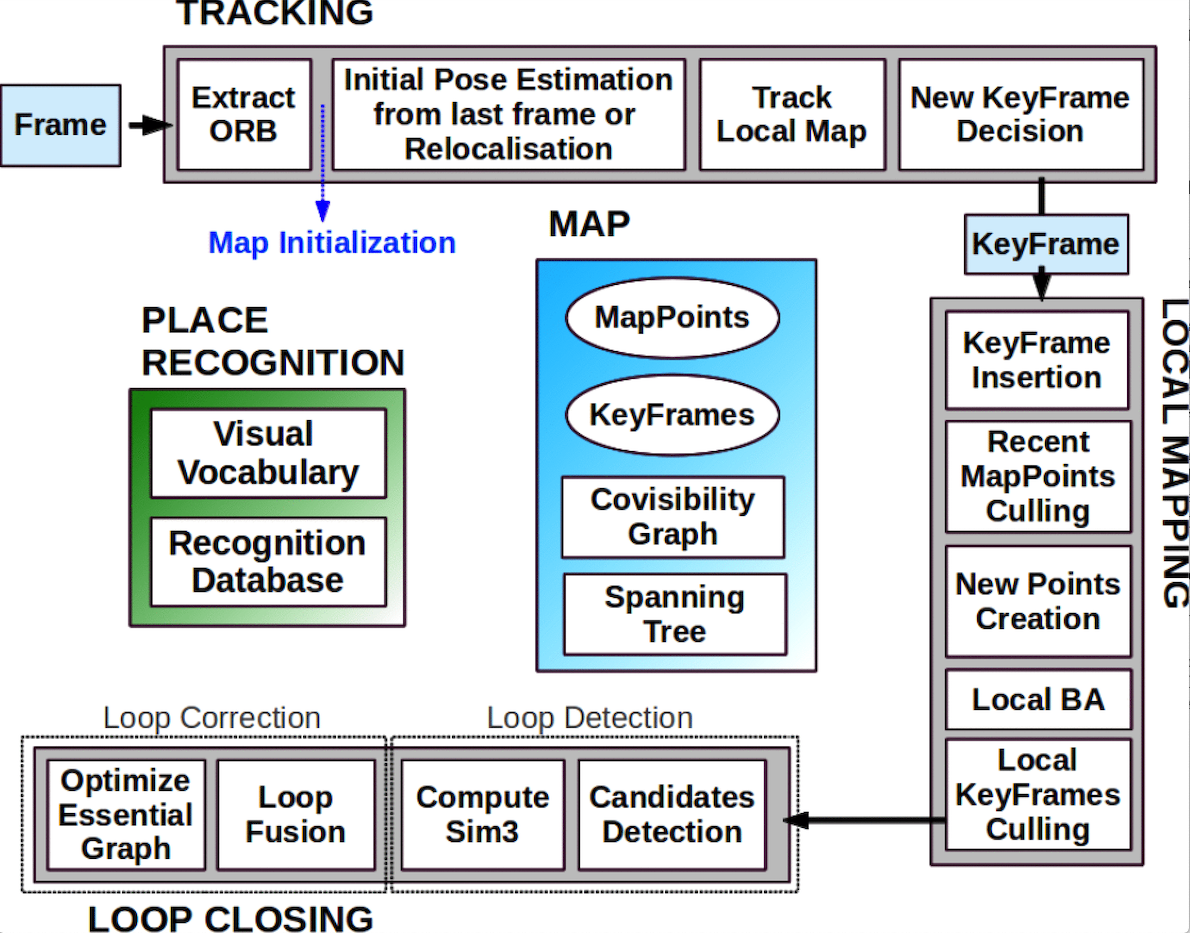
\includegraphics[width=5in]{Chapter2/ORBSLAMOverview.eps}
	\caption{ORB-SLAM system overview.}
	\label{fig:orbslamoverview} 
\end{figure}

\subsection{CORB-SLAM}
Proposed by F.Li et al. in \cite{li2017corb}, CORB-SLAM is a vSLAM algorithm focusing on  multi-robot systems. As presented in Figure \ref{fig:corbslamoverview}, the system of CORB-SLAM consists of robot-end clients and a server.
\begin{figure}[H]
	\centering
	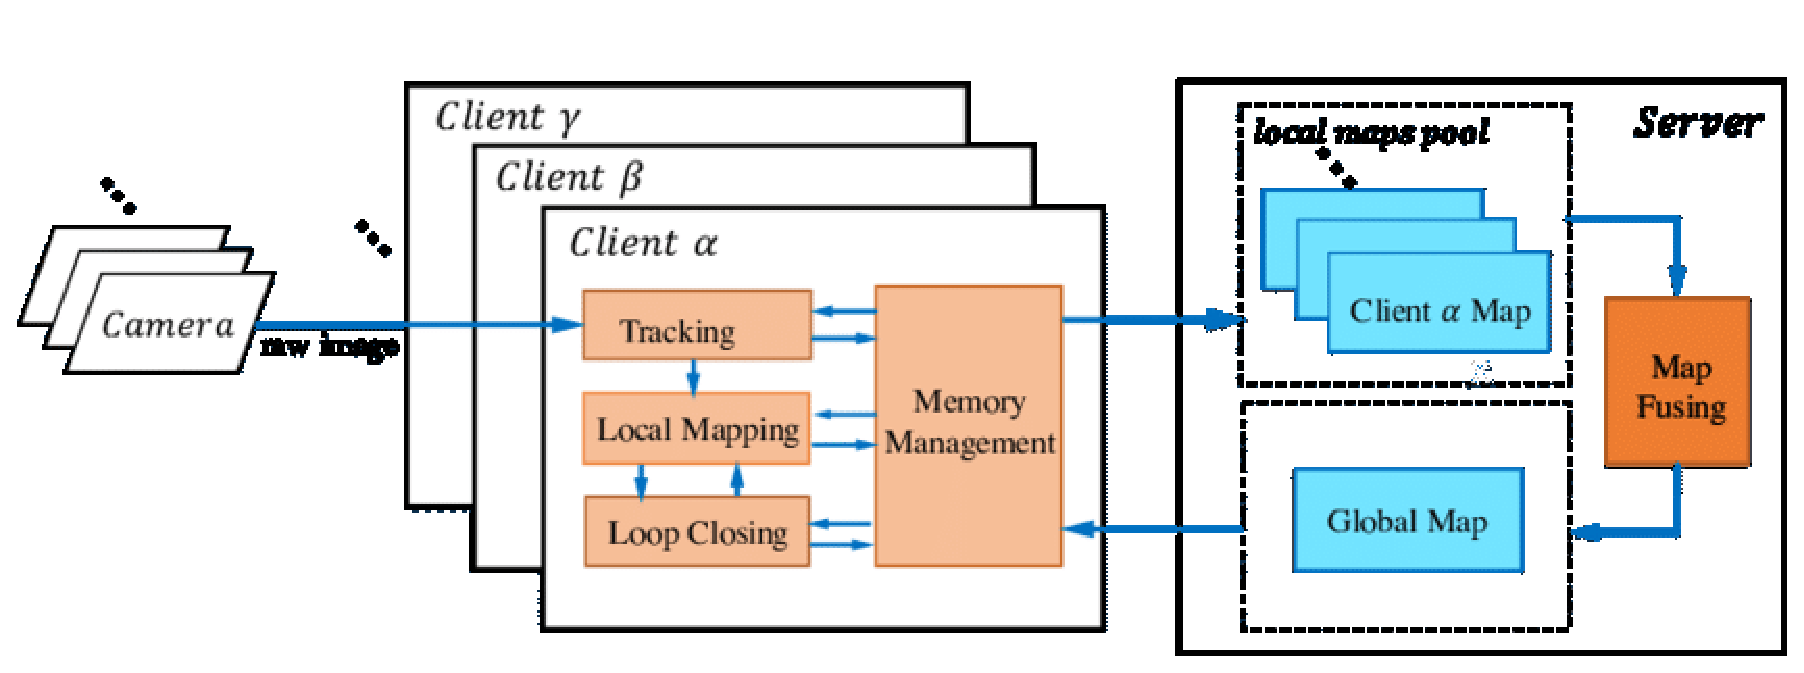
\includegraphics[width=5in]{Chapter2/CORBSLAMOverview.eps}
	\caption{The framework of CORB-SLAM system.}
	\label{fig:corbslamoverview} 
\end{figure}

\subsubsection{Robot-end SLAM Client}
The robot-end client of CORB-SLAM is an ORB-SLAM client extended to have the functionality to communicate with the server, transmitting the keyframe information, with all functions and modules in original ORB-SLAM as listed in Chapter \ref{chp:orbslam} reserved.

\subsubsection{Map Fusing in the Server}
In the server, the map fusing module receives and fuses the local maps from the clients, achieving an optimized global map. The map fusing algorithm is shown in Figure \ref{fig:corbslamserver}, including two main parts: map overlap detection and local-map fusion.

\begin{figure}[H]
	\centering
	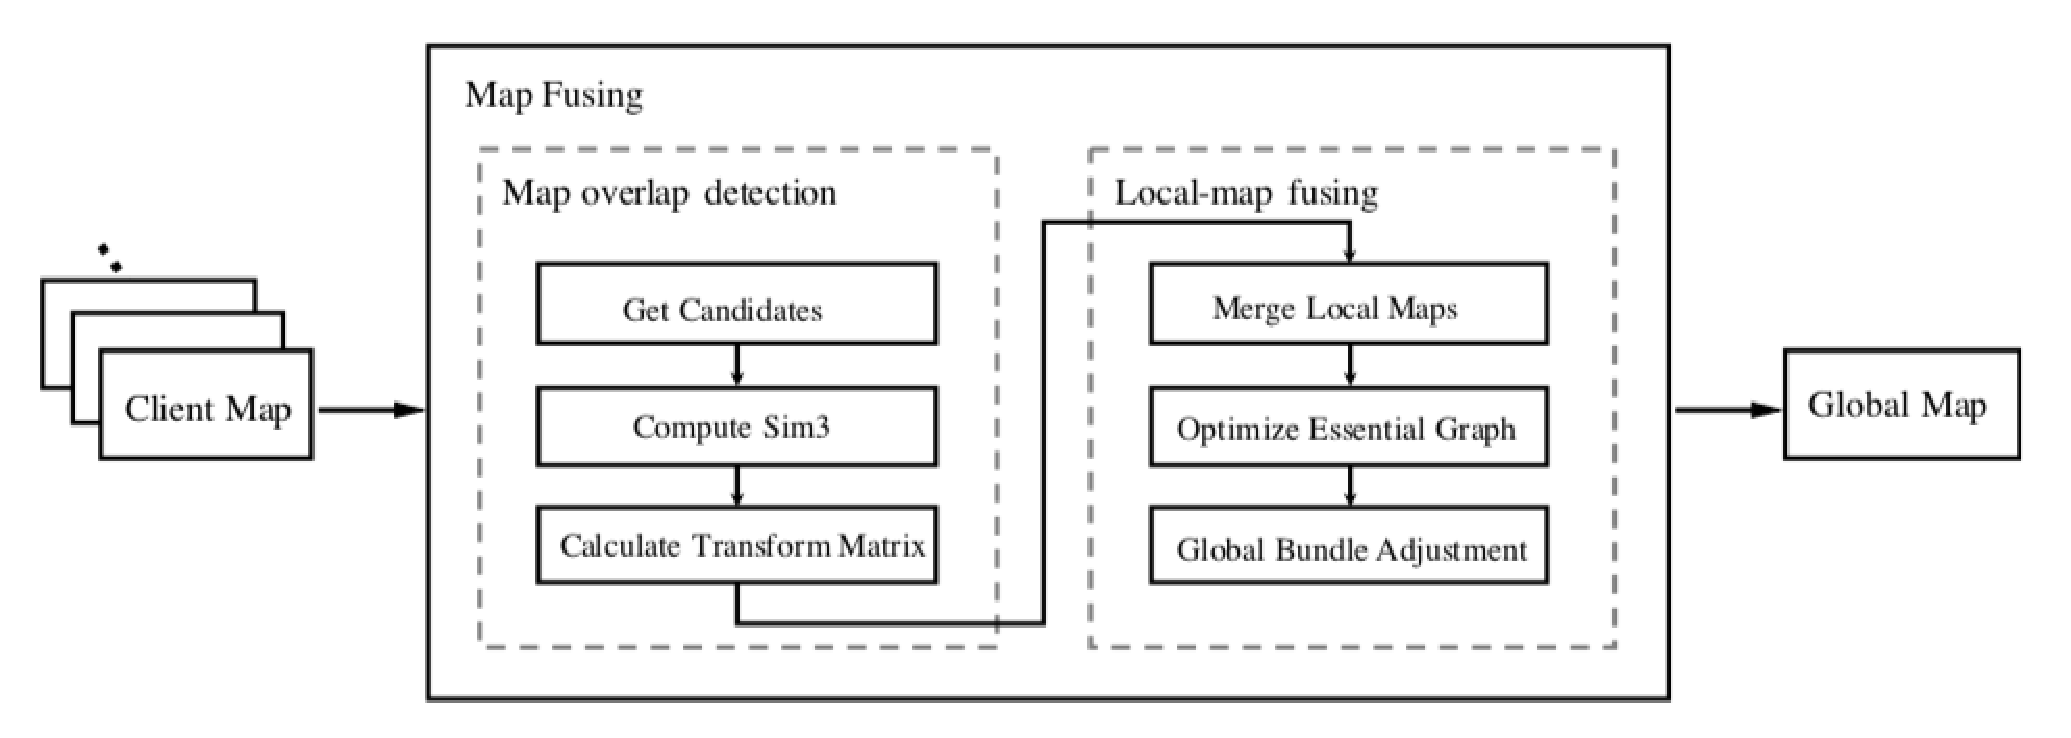
\includegraphics[width=5in]{Chapter2/corbslamserver.eps}
	\caption{The flowchart of Map Fusing module.}
	\label{fig:corbslamserver} 
\end{figure}

\begin{enumerate}[1.]
	\item Initializing global map
	
	Initially,
	
	\item Map overlap detection
	
	To
	
	\item Local map fusing 
	
	To 
\end{enumerate}

\section{Illumination Variance}

\subsection{Appearance Change From Illumination}

For vision systems concerned with localizing in known environments, dealing with appearance changes is an ongoing challenge. Appearance changes can result from several sources, such as 
\begin{inparaenum}[(i)]
	\item different lighting conditions,	
	\label{ls:appearancechange1}
	\item varying weather conditions, and
	\label{ls:appearancechange2}
	\item dynamic objects like pedestrians or vehicles.
	\label{ls:appearancechange3}
\end{inparaenum}

In previous work of Colin McManus et al. , they demonstrated how to leverage knowledge of prior 3D structure to suppress distracting objects for improved pose estimation in busy urban environments \cite{mcmanus2013distraction}, and how to cope with long-term appearance variation caused by changing weather conditions \cite{churchill2012practice}. In \cite{maddern2014illumination}, they proposed a new approach to address problem (\ref{ls:appearancechange1}) named as Illumination Variance Approach. 

Appearance change caused by different lighting conditions in (\ref{ls:appearancechange1}) is illustrated in Figure \ref{fig:shadecompare1} with pictures selected from St Lucia dataset \cite{glover2010fab}. Compared to approaches proposed in \cite{mcmanus2013distraction} and \cite{churchill2012practice}, illumination variance approach is not model-based, requiring less computational cost. And in most of applications of vSLAM, appearance changes caused by (\ref{ls:appearancechange1}) are a more common problem than (\ref{ls:appearancechange2}, \ref{ls:appearancechange3}). Therefore, how to combine illumination variance approach with multi-robot SLAM algorithms, to improve the performance of place recognition in changing illumination conditions, is the major objective focused on in this work.

\begin{figure}
	\centering
	\subfigure[pic1.]{
		\begin{minipage}[t]{0.4\linewidth}
			\centering
			\includegraphics[width=2in]{Chapter2/shadecompare1-0.eps}
			%\caption{fig1}
		\end{minipage}
	}
	\subfigure[pic2.]{
		\begin{minipage}[t]{0.4\linewidth}
			\centering
			\includegraphics[width=2in]{Chapter2/shadecompare1-1.eps}
			%\caption{fig2}
		\end{minipage}
	}
	\caption{Appearance changes caused by different lighting conditions. Pictures are selected from St Lucia dataset corresponding to the car rides recorded on 10/09/2009 at 8:45 am and at 2:10 pm}
	\label{fig:shadecompare1}
\end{figure}

\subsection{Formulation}
Illumination variance approach proposed in \cite{maddern2014illumination}, is a simple method based on only one equation computing illumination variant images. The basic idea of this approach is to map color images to an illumination invariant color space, where illumination change caused by different lighting condition like shade can be suppressed. The mapping equation
is presented in Equation \ref{eq:iifinal}.

\begin{equation}
I=\log(G)-\alpha\log(B)-(1-\alpha)\log(R)
\label{eq:iifinal}
\end{equation}

where, $R, G, B$ are the color channels of the input image, and $I$ is the resultant illumination invariant image. As shown in \ref{eq:ii1}, $\alpha$ is a parameter which depends on the peak spectral responses of each color channel ($\lambda_R, \lambda_G, \lambda_B$), which are usually available in camera specifications.

\begin{equation}
\frac{1}{\lambda_G}=\frac{\alpha}{\lambda_B}+\frac{1-\alpha}{\lambda_R}
\label{eq:ii1}
\end{equation}

Therefore, considering the peak spectral responses, $\alpha$ can be easily calculated as exposed in Equation \ref{eq:ii2}.

\begin{equation}
\alpha=\frac{(\frac{\lambda_B}{\lambda_G}-\frac{\lambda_B}{\lambda_R})}{(1-\frac{\lambda_B}{\lambda_R})}
\label{eq:ii2}
\end{equation}

The influence of applying the illumination invariant transformation is showed in Figure \ref{fig:iicompare1}.

\begin{figure}
	\centering
	\subfigure[pic1.]{
		\begin{minipage}[t]{0.4\linewidth}
			\centering
			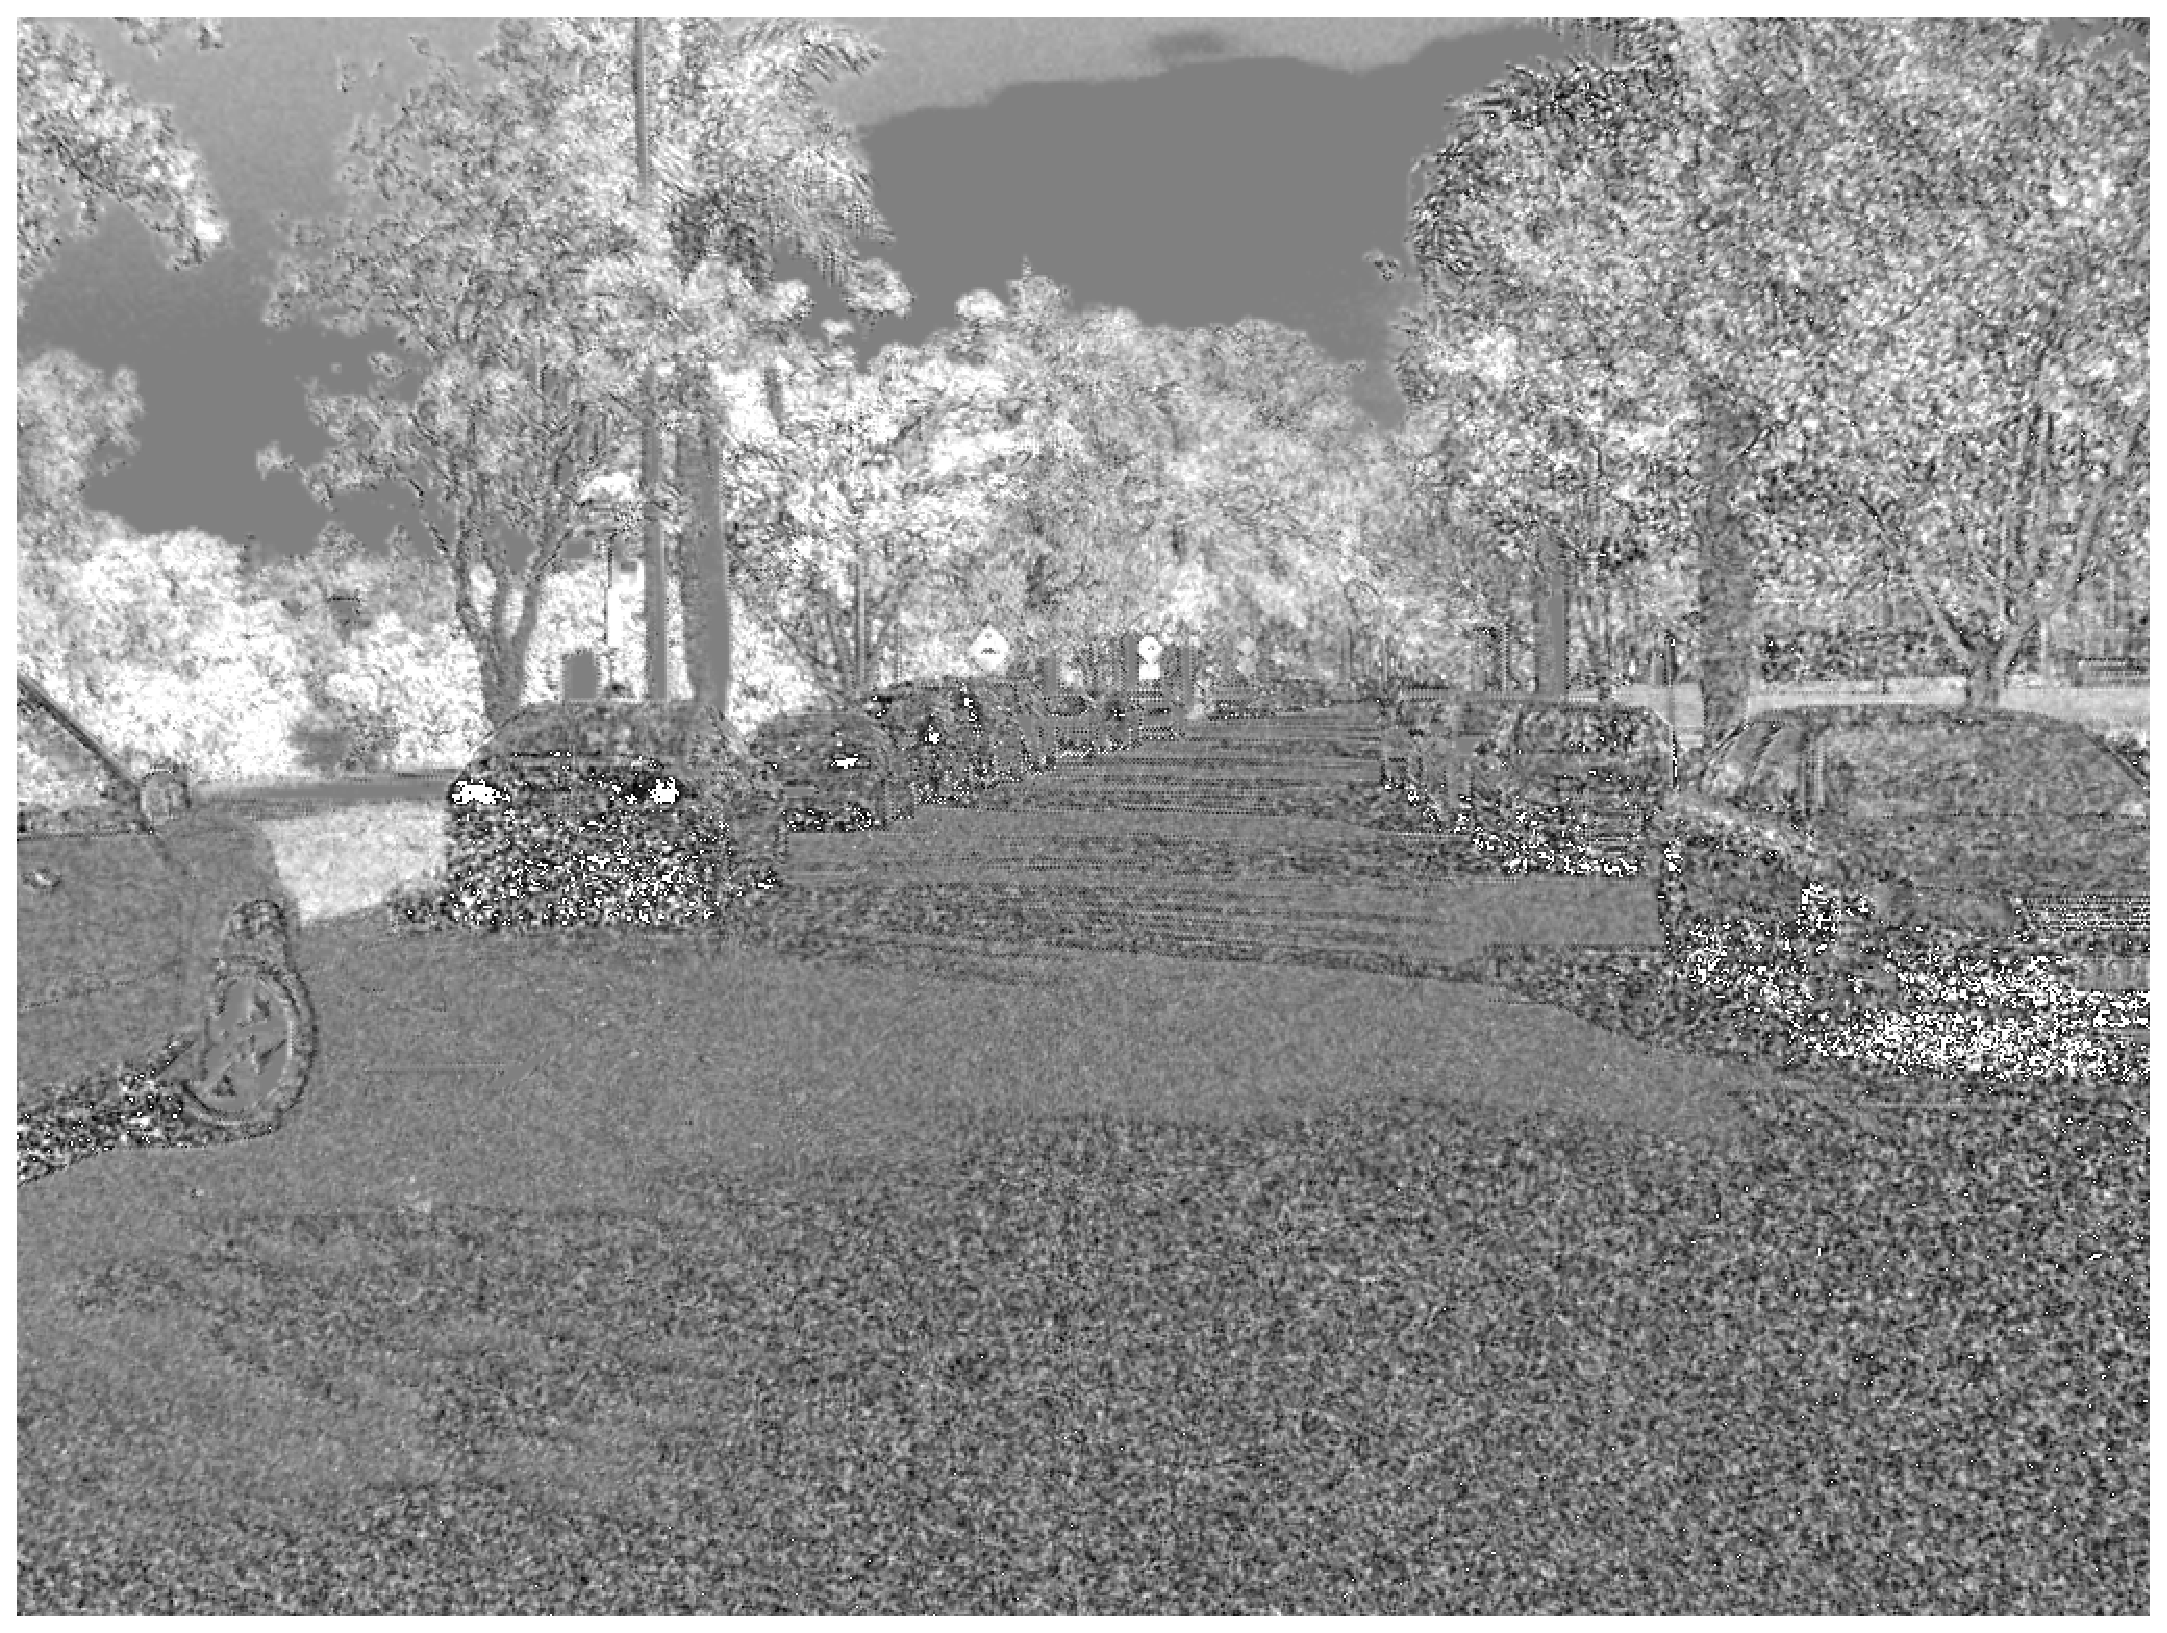
\includegraphics[width=2in]{Chapter2/iicompare1-0.eps}
			%\caption{fig1}
		\end{minipage}
	}
	\subfigure[pic2.]{
		\begin{minipage}[t]{0.4\linewidth}
			\centering
			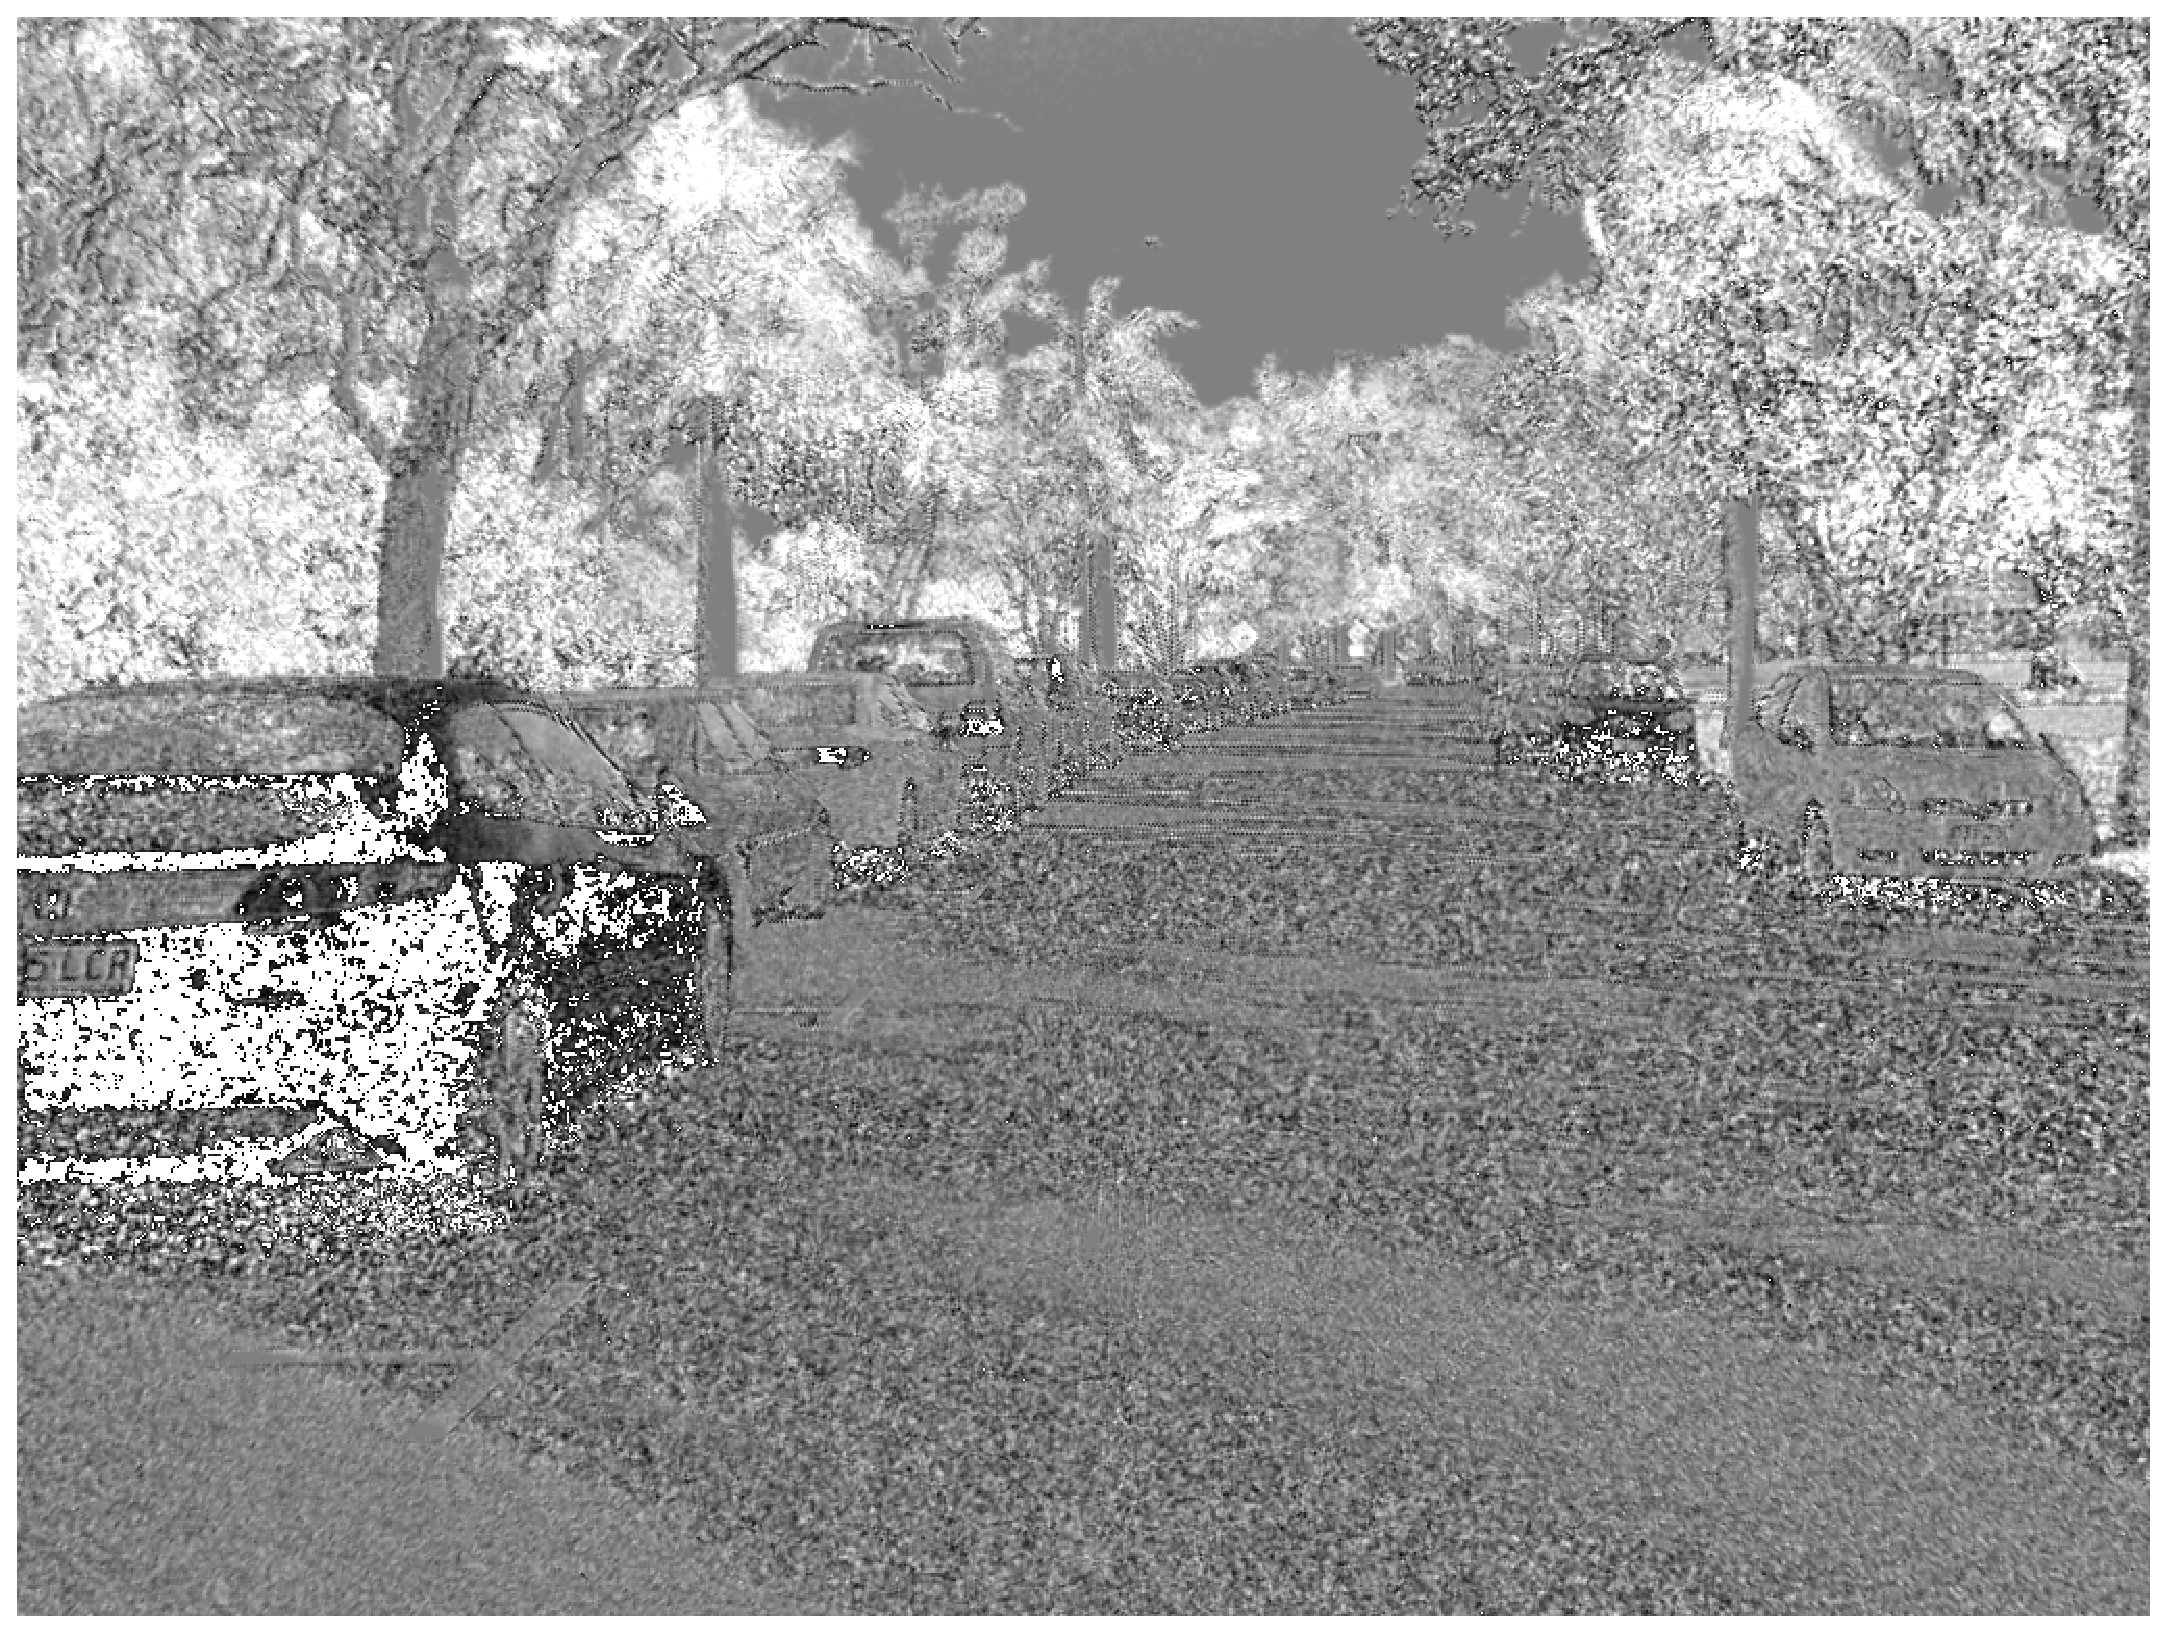
\includegraphics[width=2in]{Chapter2/iicompare1-1.eps}
			%\caption{fig2}
		\end{minipage}
	}
	\caption{An example of illumination invariance application in St Lucia dataset. It shows how this approach suppress the effects caused by sun}
	\label{fig:iicompare1}
\end{figure}

\subsection{Application of Localization}
An open source toolbox named as OpenABLE, for life-long visual localization is implemented in \cite{arroyo2016openable}. The proposed implementation in \cite{arroyo2016openable} employs the philosophy of the topological place recognition approach named ABLE introduced in \cite{arroyo2014bidirectional, arroyo2014fast, arroyo2015towards} which uses illumination variant images for relocalization.

A graphic representation about how the methodology proposed by OpenABLE is showed in Figure \ref{fig:openableoverview}.

\begin{figure}[H]
	\centering
	\includegraphics[width=5in]{Chapter2/OPENABLEOverview.eps}
	\caption{A graphic representation about how the methodology proposed by ABLE works.}
	\label{fig:openableoverview} 
\end{figure}

The limitation of illumination variance approach is the transformation process produces resultant images with low resolution because all pixel values are turned into log values. These low-resolution resultant images still can be used as the input images of visual topological localization where high resolution images are actually not needed. But in the mapping task, illumination variant images are too blurry to estimate camera motion and then reconstruct the map. Therefore, to improve the mapping performance in changing illumination conditions, rgb images and illumination variant images are both needed to perform relocalization and mapping, as the block-flow proposed in \cite{mcmanus2014shady} presented in \ref{fig:iioverview}.

\begin{figure}[H]
	\centering
	\includegraphics[width=5in]{Chapter2/COISLAMOverview.eps}
	\caption{Block-flow diagram of the combined stereo localisation approach.}
	\label{fig:iioverview} 
\end{figure}

In the framework presented in \ref{fig:iicompare1}, there is a second localizer making use of illumination invariant images in parallel with the main localization system. In \cite{maddern2014illumination}, although the metric relative poses calculated from illumination variant images tends wo be more noisy, the integrated localizer are less likely to fail if the scene appearance change is due to sunlight intensity direction or spectrum variation.

%=== END OF CHAPTER TWO ===
\newpage
